% Options for packages loaded elsewhere
\PassOptionsToPackage{unicode}{hyperref}
\PassOptionsToPackage{hyphens}{url}
%
\documentclass[
]{article}
\usepackage{amsmath,amssymb}
\usepackage{lmodern}
\usepackage{iftex}
\ifPDFTeX
  \usepackage[T1]{fontenc}
  \usepackage[utf8]{inputenc}
  \usepackage{textcomp} % provide euro and other symbols
\else % if luatex or xetex
  \usepackage{unicode-math}
  \defaultfontfeatures{Scale=MatchLowercase}
  \defaultfontfeatures[\rmfamily]{Ligatures=TeX,Scale=1}
\fi
% Use upquote if available, for straight quotes in verbatim environments
\IfFileExists{upquote.sty}{\usepackage{upquote}}{}
\IfFileExists{microtype.sty}{% use microtype if available
  \usepackage[]{microtype}
  \UseMicrotypeSet[protrusion]{basicmath} % disable protrusion for tt fonts
}{}
\makeatletter
\@ifundefined{KOMAClassName}{% if non-KOMA class
  \IfFileExists{parskip.sty}{%
    \usepackage{parskip}
  }{% else
    \setlength{\parindent}{0pt}
    \setlength{\parskip}{6pt plus 2pt minus 1pt}}
}{% if KOMA class
  \KOMAoptions{parskip=half}}
\makeatother
\usepackage{xcolor}
\usepackage[margin=1in]{geometry}
\usepackage{longtable,booktabs,array}
\usepackage{calc} % for calculating minipage widths
% Correct order of tables after \paragraph or \subparagraph
\usepackage{etoolbox}
\makeatletter
\patchcmd\longtable{\par}{\if@noskipsec\mbox{}\fi\par}{}{}
\makeatother
% Allow footnotes in longtable head/foot
\IfFileExists{footnotehyper.sty}{\usepackage{footnotehyper}}{\usepackage{footnote}}
\makesavenoteenv{longtable}
\usepackage{graphicx}
\makeatletter
\def\maxwidth{\ifdim\Gin@nat@width>\linewidth\linewidth\else\Gin@nat@width\fi}
\def\maxheight{\ifdim\Gin@nat@height>\textheight\textheight\else\Gin@nat@height\fi}
\makeatother
% Scale images if necessary, so that they will not overflow the page
% margins by default, and it is still possible to overwrite the defaults
% using explicit options in \includegraphics[width, height, ...]{}
\setkeys{Gin}{width=\maxwidth,height=\maxheight,keepaspectratio}
% Set default figure placement to htbp
\makeatletter
\def\fps@figure{htbp}
\makeatother
\setlength{\emergencystretch}{3em} % prevent overfull lines
\providecommand{\tightlist}{%
  \setlength{\itemsep}{0pt}\setlength{\parskip}{0pt}}
\setcounter{secnumdepth}{5}
\newlength{\cslhangindent}
\setlength{\cslhangindent}{1.5em}
\newlength{\csllabelwidth}
\setlength{\csllabelwidth}{3em}
\newlength{\cslentryspacingunit} % times entry-spacing
\setlength{\cslentryspacingunit}{\parskip}
\newenvironment{CSLReferences}[2] % #1 hanging-ident, #2 entry spacing
 {% don't indent paragraphs
  \setlength{\parindent}{0pt}
  % turn on hanging indent if param 1 is 1
  \ifodd #1
  \let\oldpar\par
  \def\par{\hangindent=\cslhangindent\oldpar}
  \fi
  % set entry spacing
  \setlength{\parskip}{#2\cslentryspacingunit}
 }%
 {}
\usepackage{calc}
\newcommand{\CSLBlock}[1]{#1\hfill\break}
\newcommand{\CSLLeftMargin}[1]{\parbox[t]{\csllabelwidth}{#1}}
\newcommand{\CSLRightInline}[1]{\parbox[t]{\linewidth - \csllabelwidth}{#1}\break}
\newcommand{\CSLIndent}[1]{\hspace{\cslhangindent}#1}
\usepackage{tikz}
\usepackage{pgfplots}
\pgfplotsset{compat=newest}
\usetikzlibrary{plotmarks}
\usetikzlibrary{arrows.meta}
\usepgfplotslibrary{patchplots}
\usepackage{grffile}
\usepackage{caption}
\usepackage[utf8]{inputenc}
\usepackage[doublespacing]{setspace}
\usepackage{float}
\usepackage{multirow}
\renewcommand{\topfraction}{.85}
\renewcommand{\bottomfraction}{.7}
\renewcommand{\textfraction}{.15}
\renewcommand{\floatpagefraction}{.66}
\setcounter{topnumber}{3}
\setcounter{bottomnumber}{3}
\setcounter{totalnumber}{4}
\ifLuaTeX
  \usepackage{selnolig}  % disable illegal ligatures
\fi
\IfFileExists{bookmark.sty}{\usepackage{bookmark}}{\usepackage{hyperref}}
\IfFileExists{xurl.sty}{\usepackage{xurl}}{} % add URL line breaks if available
\urlstyle{same} % disable monospaced font for URLs
\hypersetup{
  pdftitle={Planes, Trains, and Armored Mobiles: Introducing a Dataset of the Global Distribution of Military Capabilities (rDMC)},
  pdfauthor={Anonymized version},
  hidelinks,
  pdfcreator={LaTeX via pandoc}}

\title{\singlespacing Planes, Trains, and Armored Mobiles: Introducing a Dataset of the Global Distribution of Military Capabilities (rDMC)}
\author{Anonymized version}
\date{November 17, 2022}

\begin{document}
\maketitle
\begin{abstract}
\singlespacing \noindent This article introduces a new dataset on the disaggregated military capabilities states possess from 1970 -- 2014. While practitioners have long recognized the importance of what weapons states own, scholars have largely examined surrounding questions in piecemeal fashion due to data limitations. The Distribution of Military Capabilities (rDMC) dataset identifies the weapons portfolios of states over the past half century at various levels of aggregation suitable to a wide variety of research questions. This paper begins by explaining the value of collecting data on disaggregated national military capabilities, the data's scope, and the data collection process. I then identify some initial trends about changes in the distribution of military capabilities across states. I conclude by identifying future research use of the data as both a dependent and independent variable. These data allows scholars to better investigate both international questions concerning power projection, military innovation, and conflict outcomes as well as domestic questions like coup risks, use of force decisions, and interest group lobbying.
\end{abstract}

\newpage

\hypertarget{introduction}{%
\section{Introduction}\label{introduction}}

The military capabilities states possess are an important instrument of military power, and consequently national power. Yet existing work on how states exercise military power are limited in empirical identification to coarse measures like military spending or military personnel. Not all soldiers are created equal, and much has been said about the problems of measuring military power using military spending figures (Perlo-Freeman 2017) or aggregate measures like the Composite Index of National Capabilities (CINC) (Beckley 2018; Carroll and Kenkel 2019). I define military capabilities as the technologies and weapons that states can use in combat operations. While military capabilities are but one of only many components of military power, its effects are significant, if hotly debated (Lieber 2005; R. Brooks and Stanley 2007). Inconsistent findings about the role of capabilities in conflict stem not from the fact that they do not matter, but rather they have been improperly identified and coarsely measured (van Creveld 2005).

This paper contributes to ongoing research about the technological dimension of military power by producing the first comprehensive dataset of the distribution of military capabilities across all states from 1970 -- 2014. Disaggregating military power into its component parts is an important, yet underdeveloped, enterprise. While aggregate military spending may help differentiate large and globally capably militaries from smaller ones, it risks conflating differences in the \emph{composition} of nominally equivalently sized militaries. The composition of a state's military may influence its power projection and warfighting capabilities in some conflicts, but not others (Gartzke and Lindsay 2020), and the relationship between the military capabilities a country could acquire, actually possesses, and subsequently uses in a contest could shed light on contrasting findings about the impact of military capabilities on international affairs (Douglass and Gannon 2019).

This paper proceeds as follows. Section \ref{the-case-for-disaggregating-defense} identifies the role that military capabilities play as both a dependent and independent variable in the study of international politics. Section \ref{existing-measures-of-military-capabilities} outlines existing empirical work on the military capabilities states possess. Section \ref{the-rdmc-dataset-scope-and-data-generating-process} outlines the scope of the newly produced Distribution of Military Capabilities (rDMC) dataset and section \ref{data-collection-and-formats} briefly describes the data collection process. Section \ref{global-trends} identifies some initial trends in variation in the distribution of military capabilities across time and space and Section \ref{conclusion} concludes.

\hypertarget{the-case-for-disaggregating-defense}{%
\section{The case for disaggregating defense}\label{the-case-for-disaggregating-defense}}

One of the most political aspects of international security for policymakers concerns what military capabilities a state should possess. What a states produces and omits in its defense portfolio reflects its political priorities in ways that economic considerations alone cannot explain (Caverley 2007). As then-Senator Joseph Biden (2008) remarked regarding domestic economic policy during his vice presidential campaign, ``{[}d{]}on't tell me what you value. Show me your budget, and I'll tell you what you value.'' This also holds true in the military context, where disconnects concerning a state's budget and alleged priorities are missed by scholars looking at top-line spending figures. Despite decades of concern about a Chinese invasion of Taiwan, it was not until 2017 that China began investing in the amphibious assault capabilities that are necessary for that threat to actually be carried out (Office of the Secretary of Defense 2018, 95--99). This important fact was missed by many who looked only at the size of China's defense budget, rather than what capabilities they actually possessed.

The wide body of literature studying war has recognized that international affairs is influenced by \emph{how} states fight (Gannon 2022). The United States' decision to adopt a more capital-intensive military concentrated in a few high-value weapons may explain its relatively infrequent uses of force, given its high military spending (Fordham 2004), while states with combined arms militaries are able to end civil conflicts more rapidly (Caverley and Sechser 2017). Looking at specific military domains, states with capable navies fight wars further from their borders (Crisher 2017) while those conducting aerial mobilizations fail at demonstrating resolve (Post 2019). Concerning intrastate conflict, access to armored fighting vehicles helped the Yemeni Army secure the capital during the 1962 coup (Albrecht and Eibl 2018, p 319) and well-resourced armies are better able to negotiate with their civilian counterparts in a way that shapes civil-military relations (Kadercan 2014).

Domestically, the portfolio of military capabilities also informs questions outside the traditional scope of international security. Tension between political budget constraints and military security desires gets to the heart of the role that military capabilities play in furthering our understanding of national politics (Cappella Zielinski 2016). Partisan politics is intricately tied to the composition of a state's military, as the Cold War witnessed a preference among Republican US presidents for funding strategic forces while Democratic presidents funding conventional forces during the Cold War (Fordham 2002). In the 1960's, the US developed the F-111 fighter-bomber and C-5A jumbo transport aircraft to keep production lines for the four major aerospace corporations funded, demonstrating how patterns of weapons acquisition can tell us about the role of domestic industry in political decisions (Kurth 1972).

\hypertarget{existing-measures-of-military-capabilities}{%
\section{Existing measures of military capabilities}\label{existing-measures-of-military-capabilities}}

The combination of capabilities that comprise a military's toolkit determine the operations it undertakes, the types of threats it can credibly make, and the consequences of resorting to force. Military means likely matter, but proving that they do (and if so, the degree and circumstance) is an impossible endeavor without empirical data on the distribution of those means across time and space. Despite the importance of disaggregated military capabilities and a recognition of the shortcomings of aggregate measures for explaining concepts of interest, most current research uses measures only of the \emph{size} of state militaries.\footnote{Of course, these two are not synonymous. Military capabilities are only one component of military spending and the cost of labor is a large component of military spending (Whitten and Williams 2011).} National militaries are primarily quantified and compared by military spending levels or, in rarer cases, military personnel counts. Yet, defense dollars don't tell us what capabilities a state can actually use during a conflict. Despite its frequent use, data on military spending also poses known problems for quantitative cross-national and temporal comparison (Perlo-Freeman 2017). Since there are no common definitions about what constitutes military spending, some states measure things like pension and R\&D while others do not (Amara and Paskevics 2010). Exchange rates are often used to standardize all spending to the same currency, but with ill-information applications of domestic purchasing power (Fontanel 1996). Difficulty accounting for inflation and budget cycles also dramatically impacts inferences drawn from different data sources (Lebovic 1999). The IMF, UN Office for Disarmament Affairs, US Bureau of Arms Control, Verification, and Compliance, International Institute for Strategic Studies (IISS), and Stockholm International Peace Research Institute (SIPRI) all produce annual military spending estimates using different estimating procedures, primary sources, and preparation methods (Brzoska 1981), meaning findings from one data source are often not supported using comparable data from another source (Boniface 1995). Since the cost of military platforms has increased over time, having data on the actual platforms helps get around the problems of accounting for military ``purchasing power'' over time.

Research on variation in the \emph{composition} of militaries remains nascent. Scholars have noted ``there is a lack of knowledge about variation between states in their behavior on armaments policy decisions'' because of problems empirically identifying the military capabilities states possess (Mawdsley 2018). Recent works that disaggregate military capabilities have narrowed their focus to a small set of platforms like mechanized vehicles (Lyall and Wilson 2009; Sechser and Saunders 2010), strategic lift aircraft (Kupchan 1988), principal naval platforms (Crisher and Souva 2014), or fighter jets (Saunders and Souva 2020) or to a small set of countries like great powers (S. G. Brooks and Wohlforth 2016) or China and its regional rivals (Beckley 2017). Even the most detailed of these are selective in their disaggregation; Saunders and Souva (2020) do not include bombers, air transport, or support aircraft, Sechser and Saunders (2010) omit helicopters, and Souva (2023) aggregates all capabilities to five categories (nuclear weapons, naval tonnage, air power, armor, and ballistic missiles) . The primary reason for this relatively limited use of fine-grained high-quality data is difficulty in converting the data to an easily-usable format and standardizing it across countries and years. rDMC aims to overcome all of these problems in being a massively expanded dataset that better enables systematic analysis across time, space, and military capability.

\hypertarget{the-rdmc-dataset-scope-and-data-generating-process}{%
\section{The rDMC dataset: scope and data generating process}\label{the-rdmc-dataset-scope-and-data-generating-process}}

This paper introduces the first comprehensive dataset of disaggregated military capabilities measures as the annual count of military capabilities owned by 184 countries from 1970 -- 2014. By military capabilities, I mean the technologies, weapons, and equipment that states can use in combat operations, excluding small arms like handguns and rifles and also excluding munitions and bombs for which annual data is unreliable.\footnote{See the section ``Defining military capabilities'' in the codebook for a more detailed definition of military capabilities.} The data were coded by a team of 39 undergraduate coders from four universities over the past five years, resulting in 354,405 unique observations. Figure \ref{fig:missingness} shows the percent of years coded for each country. 54\% of countries have no missing data across the entire time span, with the median country having data available for 95\% of its years and the mean country having 88\% coverage.\footnote{I use percent of years since not all countries exist across the entire duration of the data. 100\% of Slovenia is covered, for example, because data exists for all 22 years since since it established independence in 1991.} The data and all code used to process, clean, and analyze the data are publicly available at (website redacted).

\begin{figure}
\centering
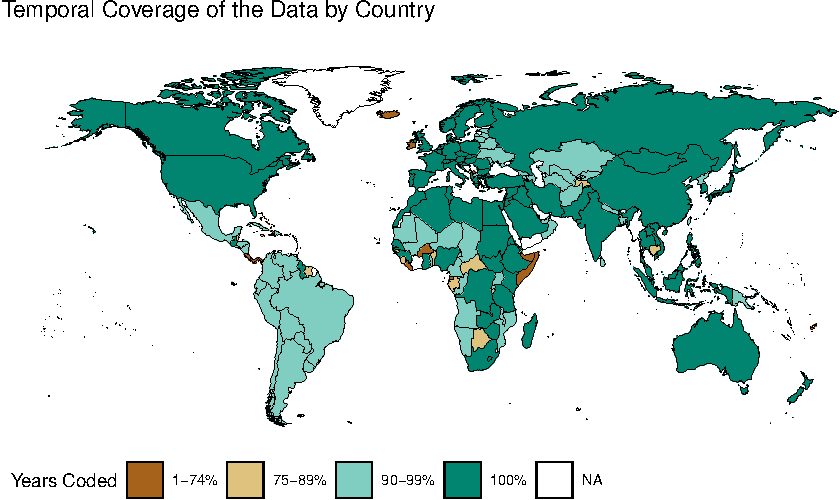
\includegraphics{figures/missingness-1.pdf}
\caption{\label{fig:missingness}Missingness map illustrating the extent of available data on state military capabilities. Almost all states have data for at least 90\% of the years they were recognized state entities.}
\end{figure}

The data comes from the annual International Institute for Strategic Studies (IISS) Military Balance reports (n.d.). Policymakers frequently use the IISS Military Balance to guide their decisions. The former Supreme Allied Commander of NATO, Admiral James Stavridis, said ``throughout my career, I have relied extensively on The Military Balance produced so expertly by the IISS. It is the''go to'' source for serious analysts and warriors facing real world challenges.'' Former US Army General Petraeus describes it as ``the go-to source of unclassified, independent information on defense capabilities around the world''. Similarly, former US Secretary of Defense Robert Gates noted it ``provides essential facts and analysis for decision-makers and for better informed public debate'' and former US Secretary of Defense Leon Panetta remarked it is ``widely recognised as the best unclassified source of defense information on personnel, equipment and budgets for every country.''\footnote{Quotes come from \href{https://www.iiss.org/publications/the-military-balance}{IISS Testimonials}}

As with much data in international affairs, concerns about data quality and accuracy remain salient. The extensive use of the IISS Military Balance by policymakers as well as by other scholars gives confidence in its accuracy and allows for the data codings to be validated. Most of this academic work has used IISS data on military spending (Wohlforth 1999; Greenhill and Major 2007) or personnel (Stanton 2013; Gaibulloev et al. 2015). Recent works by Lyall and Wilson (2009), Sechser and Saunders (2010), S. G. Brooks and Wohlforth (2016), and Caverley and Sechser (2017) use detailed information from the IISS Military Balance on platforms like mechanized vehicles and power projection platforms. The accuracy of the data has also been double checked in instances where there are reliable primary source data from government reports. New Zealand, for example, publishes annual reports on the military's performance targets that describe the resources at the military's disposal (Alexander, King, and Robert 2002). Although such data is not available for all countries nor for all years, checking the data where possible provides face validity about its accuracy.

\hypertarget{data-collection-and-formats}{%
\section{Data Collection and Formats}\label{data-collection-and-formats}}

The first step of the data collection process creates a consistent typology of military equipment types, equipment names, and unit names. I create three versions of the data. The first, \emph{rDMC raw}, organizes military equipment true to the original IISS categorizations. The second and third, \emph{rDMC long} and \emph{rDMC wide} produce a new more aggregated classification of military capabilities. The \emph{rDMC} codebook defines the military capabilities included. Table \ref{table:categories} shows the unique values that exist at each nested level, and how that is aggregated in the final classification. A detailed description of the three different data versions follows.

\begin{singlespace}   
\begin{table}[h]
\centering              
\caption[Categories of military capabilities]{Description of unit of analysis and variables in the different versions of the rDMC dataset.}
  \begin{tabular}{|c|c|c|c|}
    \hline
    \textbf{Data Version} & \textbf{Unit of Analysis} & \textbf{N} & \textbf{Variables} \\
    \hline
    Raw & Country-year-military unit & $354,405$ & Service, disaggregated category, count \\
    \hline
    Long & Country-year-military technology & $423,486$ & Aggregate category, count \\
    \hline
    Wide & Country-year & $6,535$ & Technologies \\
    \hline
\end{tabular}
\label{table:categories}
\end{table}
\end{singlespace}

\hypertarget{rdmc-raw}{%
\subsection{rDMC raw}\label{rdmc-raw}}

\emph{rDMC raw} provides an unaltered version of the original data without subjective coding decisions or equipment categorizations. IISS categorizes military capabilities in five descending levels: equipment types, equipment subtypes, equipment names, equipment subnames, and unit names.\footnote{While these 5 classifications levels are produced by IISS, their labels are the author's.} An example is provided in Figure \ref{table:equipment}. Equipment type involves the most aggregate categorizations (``aircraft'' or ``armored fighting vehicles''). Equipment names are the next primary IISS categorization (``transport'' or ``fighter'' aircraft). Subtype and subname are auxiliary classifications that exist for some, but not all technologies (designations of ``light'', ``medium'', and ``heavy'' transport aircraft or ``FFM'' frigates with surface to air missiles). Lastly, the unit names identifies specific models (``M1A1 Abrams'' tank). \emph{rDMC raw} is the only version of the data that provides this unit-level information.\footnote{Standardizing string variables across unit names is a challenging endeavor that will be advanced in future iterations of the data. For more information about using the unit-level information in \emph{rDMC raw}, see the appendix.} In this way, scholars can used the disaggregated data to identify, for example, how many countries have Aim-9 Sidewinder missiles in each year. Comparisons across country and year are possible, provided the research is careful in noting different naming conventions at the unit level.\footnote{For example, entries exist for the ``AIM-9'', ``AIM-9 Sidewinder'', ``Aim-9'', and ``Aim-9 Sidewinder'', which all refer to the same capability but with differences in capitalization and punctuation. rDMC 2.0 will standardize the unit-level names, but the time-intensive nature of that effort means it will not be completed for some time.}

\begin{singlespace}   
\begin{table}[h]
\centering              
\caption[Equipment sample]{Wquipment categories example from rRMD \textit{raw}. Non-equipmented category columns omitted.}
  \begin{tabular}{|c|c|c|c|c|}
  \hline
  \textbf{Type} & \textbf{Subtype} & \textbf{Name} & \textbf{Subname} & \textbf{Unit name} \\
  \hline
  Aircraft & NA & TPT & light & Cessna 208B \\
  \hline
  Principal surface combatants & frigates & FFM & NA & Mourad Rais \\
  \hline
  Armoured fighting vehicles & NA & MBT & NA & M1A1 Abrams \\
  \hline
\end{tabular}
\label{table:equipment}
\end{table}
\end{singlespace}

4. If I understand correctly, the author will provide the disaggregated data so that users can either create their own aggregations or just record which countries have a specific type of air-to-air missile. Is that correct? In other words, can researchers determine the number of countries that have Aim-9 Sidewinder missiles from this data set? Would researchers be able to learn how many Aim-9\textquotesingle s each country has?

\emph{rDMC raw} can be used to examine questions concerning topics like combat effectiveness, arms sales, and interest group lobbying. Scholars have identified the challenges of identifying observable ex-ante proxies for the military effectiveness of particular platforms (R. Brooks and Stanley 2007). Biddle (2005, 135) uses the age of a military capability as a proxy for its effectiveness. During Operation Desert Storm, the average date of introduction for US weapons was 1974 while Iraq's was 1962, with the assumption being that newer capabilities were more advanced. But until now, broader measures of the age of different components of a state's military portfolio have remained un-examined. Figure \ref{fig:mbt-invention} shows a broader comparison of the age of introduction for each main battle tank in the data as well as its last recorded year in service. The year of introduction is identified as the first year in which at least one state possessed that type of tank.\footnote{Since the data starts in 1970, tanks first deployed in 1970 most likely represent models developed before then. A more thorough analysis would track down the actual deployment date for each tank model, rather than relying on their deployment date as done here. Importantly, the data does distinguish between different platform upgrades, differentiating an F-16A from an F-16B in most cases.} Scholars could broaden Biddle's analysis beyond the Gulf War by identifying differences in predicted battlefield performance across generations of all types of technologies. This exercise also serves as a method of data validation, as the data are consistent with historical accounts concerning the development of many of these tanks like the M1 Abrams entering service in 1980 and the Japanese Type 10 being developed in 2012 (Ludeke 2018).

\begin{figure}
\centering
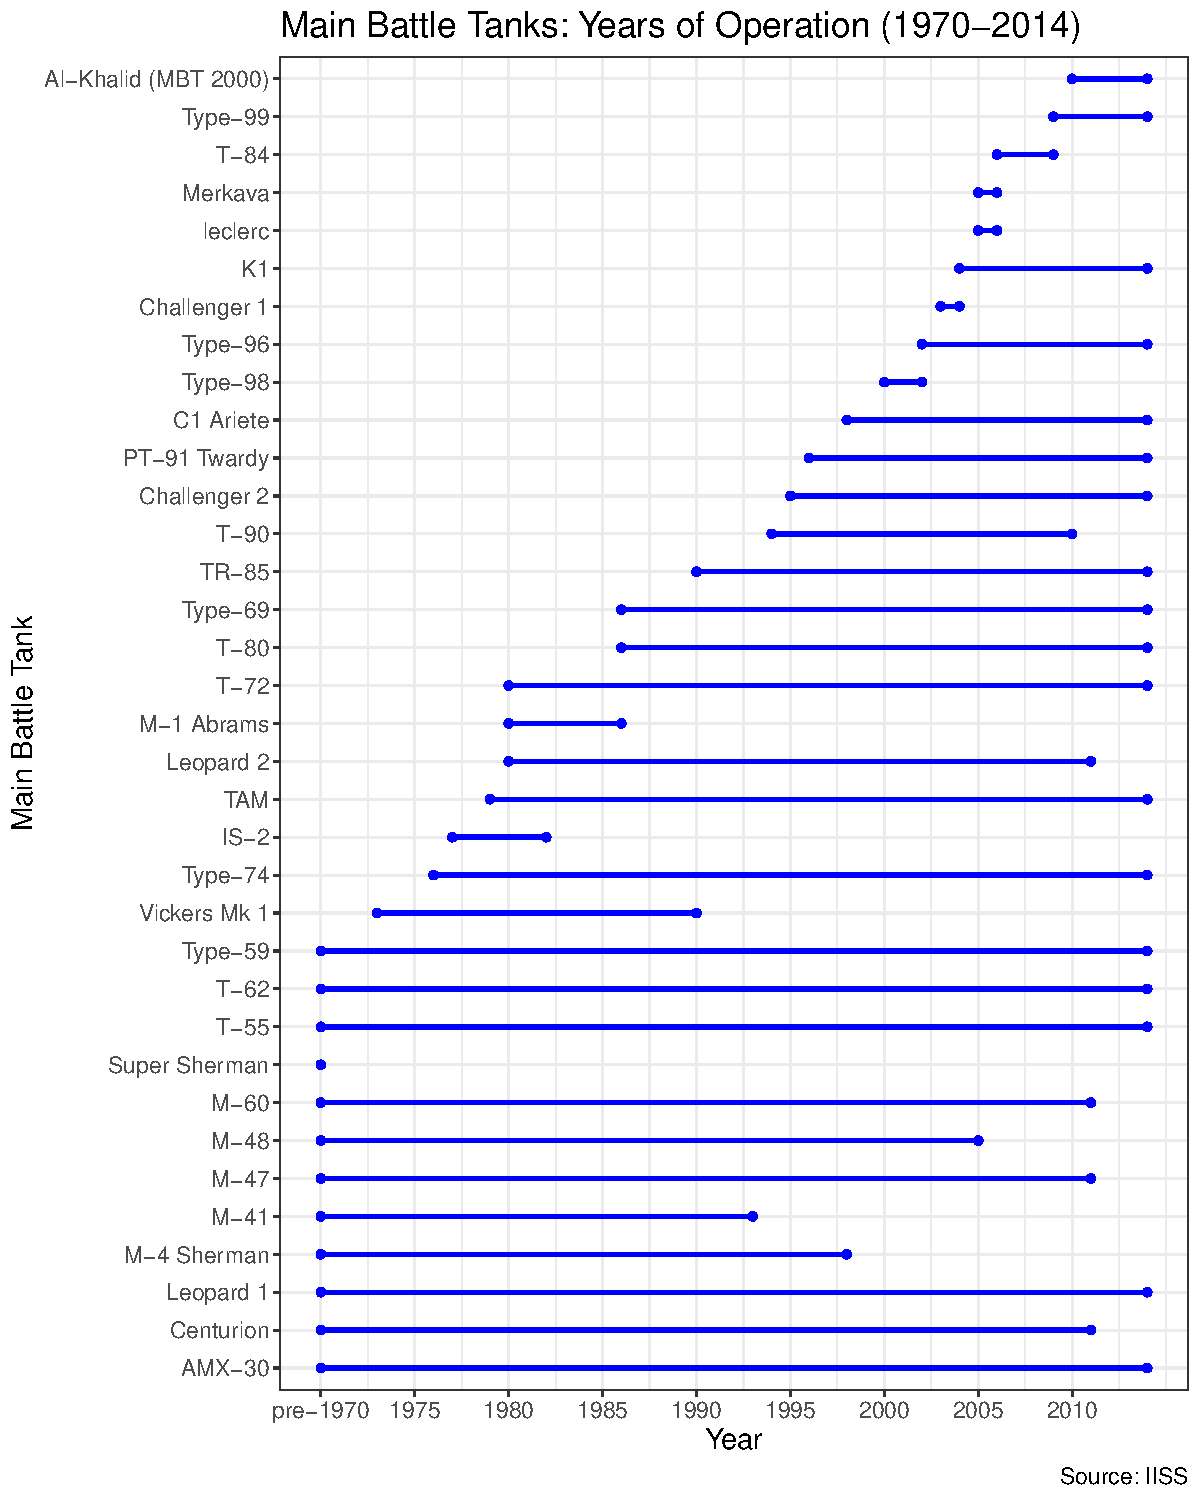
\includegraphics{figures/mbt-invention-1.pdf}
\caption{\label{fig:mbt-invention}The first year in which each type of main battle tank was deployed by any state. The figure is organized chronologically, with the newest main battle tanks at the top.}
\end{figure}

\hypertarget{rdmc-long-and-rdmc-wide}{%
\subsection{rDMC long and rDMC wide}\label{rdmc-long-and-rdmc-wide}}

\emph{rDMC long} and \emph{rDMC wide} provide a new, aggregated typology of national military capabilities.\footnote{\emph{rDMC long} and \emph{rDMC wide} are identical in terms of scope and values and differ only in the unit of analysis. In \emph{rDMC long} the unit of analysis is the country-year-technology while in \emph{rDMC wide} the unit of analysis is the country-year. They are both provided to simplify the process of merging with existing datasets much like the Alliance Treaty Obligations and Provisions (ATOP) provides alliance data at various units of analysis (Leeds et al. 2002).} The 69 categories that comprise the technologies are shown in Figure \ref{fig:dendrogram}. These categories were chosen because they represent weapons categories commonly recognized and used by states in arms reduction agreements like the Treaty on Conventional Armed Forces in Europe (CFE). As a result, national records are most consistent and accurate at this level of analysis since those records were used during international negotiations. The resulting data provides a count of, for example, ``aircraft -- transport'' for every country with a value that is the sum of all the rows in \emph{rDMC raw} that had the original 5-level categorizations that match the new ``aircraft - transport'' category.

\begin{figure}
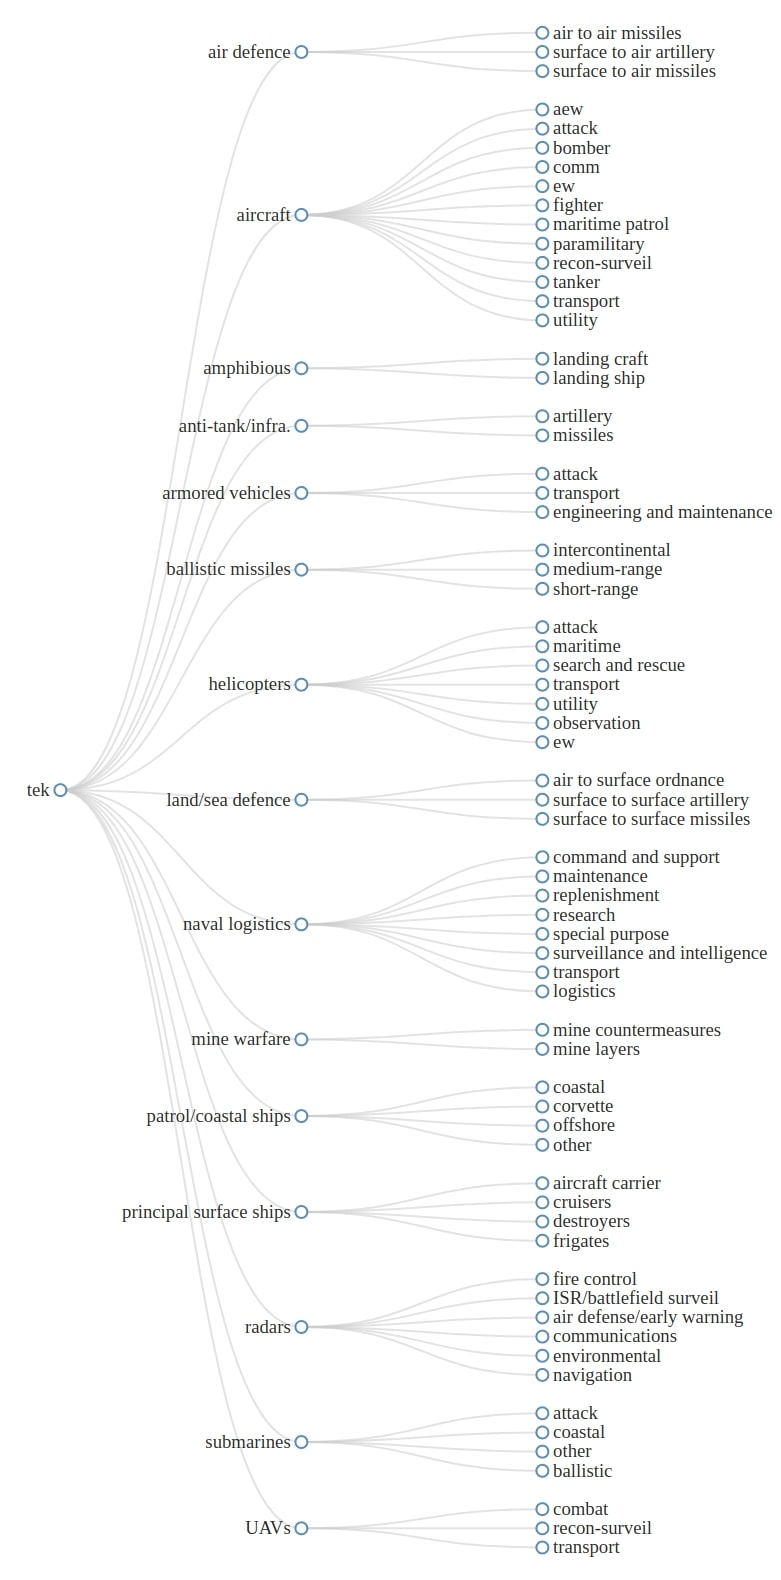
\includegraphics[width=10.85in]{figures/dendrogram_subjective_full} \caption{Description of the disaggregated technology categories used to compute the distribution of military capabilities.}\label{fig:dendrogram}
\end{figure}

Empirically, this new typology is helpful because the technology categories are definitionally uniform across the data sample. Unlike \emph{rDMC raw}, the new typology is standardized so it is consistent across country and year, thus simplifying time series-cross sectional comparisons. Where inconsistencies arise, transparent coding decisions were made with reference to external sources documented in the code repository. This ensure that, for example, the C-130H Hercules is always listed with an equipment type coding of `aircraft' and an equipment name coding of `transport (TPT)'.\footnote{There are cases where an equipment's category changes in ways the data maintains. For example, many aircraft and helicopters are phased out by being shifted to non-combat roles like training before they are fully retired. A country may thus experience a decrease in combat aircraft and an increase in training aircraft from one year to the next without the actual aircraft they possess changing.} Aggregating the technology categories also reduces the sparseness of a dataset that is already zero-inflated. While most country-years possess armored fighting vehicles, not all possess every kind of armored fighting vehicle (main battle tanks, armored personnel carriers, armored infantry fighting vehicles, and reconnaissance vehicles) let alone each of the 1,759 distinct units categorized as ``armored fighting vehicles''. That is not to say that every type or model is the same; but those distinctions present computational challenges for broad international relations questions. Scholars interested in making those distinctions are advised to use the \emph{rDMC raw} version of the data.

There are, of course, many ways to categorize technologies depending on the research question. Disagreement over the categories produced by \emph{rDMC long} and \emph{rDMC} \emph{wide} are remedied by the existence of \emph{rDMC raw} that can be used by scholars to produce their own categorizations. ``Aircraft -- transport'' and ``helicopters -- transport'' could be considered somewhat interchangeable to those interested in a state's ability to move personnel and material. Alternatively, ``helicopters -- transport'' and ``helicopters -- search and rescue'' may be reasonably combined if studying arms sales or military base location given their similar physical make-up. In other cases, categories could be further \emph{dis}aggregated. The category ``aircraft -- maritime patrol'', for example, include anti-submarine warfare, anti-surface warfare, and maritime reconnaissance which all ``patrol'' different areas of the sea. Rather than try to create and justify a single definitive ontology of military technologies, the data are constructed so that all aggregations are transparent and modular. By simply selecting new aggregation categories, scholars can produce their own counts with different categories to produce a new dataset consistent with classifications that suit their research question.

\hypertarget{global-trends}{%
\section{Global Trends}\label{global-trends}}

This section identifies some descriptive trends in military capabilities across time and space to highlight ways scholars can use these data in their own research.

\hypertarget{technological-trends-across-time}{%
\subsection{Technological Trends Across Time}\label{technological-trends-across-time}}

\emph{rDMC} can shed light on topics like military diffusion and military effectiveness by providing empirical data about how militaries change over time. For example, research on military diffusion has argued that the rate at which weapons technologies spread to other states around the globe influences the likelihood of war (Bas and Coe 2012) as well as its outcomes (Zarzecki 2002). Yet research on how and when diffusion occurs has been empirically limited to particular technologies, states, or time periods (Horowitz 2010; Gilli and Gilli 2014). Providing the first comparison across all military technologies and states over the past half century, Figure \ref{fig:common-teks} shows the number of countries that possessed each military technology in a given year. Although there is a general global trend of innovation, it is not constant across military capabilities. The number of states possessing certain capabilities like surface-to-air and surface-to-surface missiles has increased dramatically since 1970. This is in marked contrast to ballistic missiles, where their diffusion over time has been much more limited.\footnote{For existing work on missile proliferation, see Kahn and Horowitz (2022) and Schwartz and Horowitz (2021).} Fighter aircraft have increasingly diffused at a more rapid rate than bombers, despite a seeming decline in ground attack aircraft.

\begin{figure}
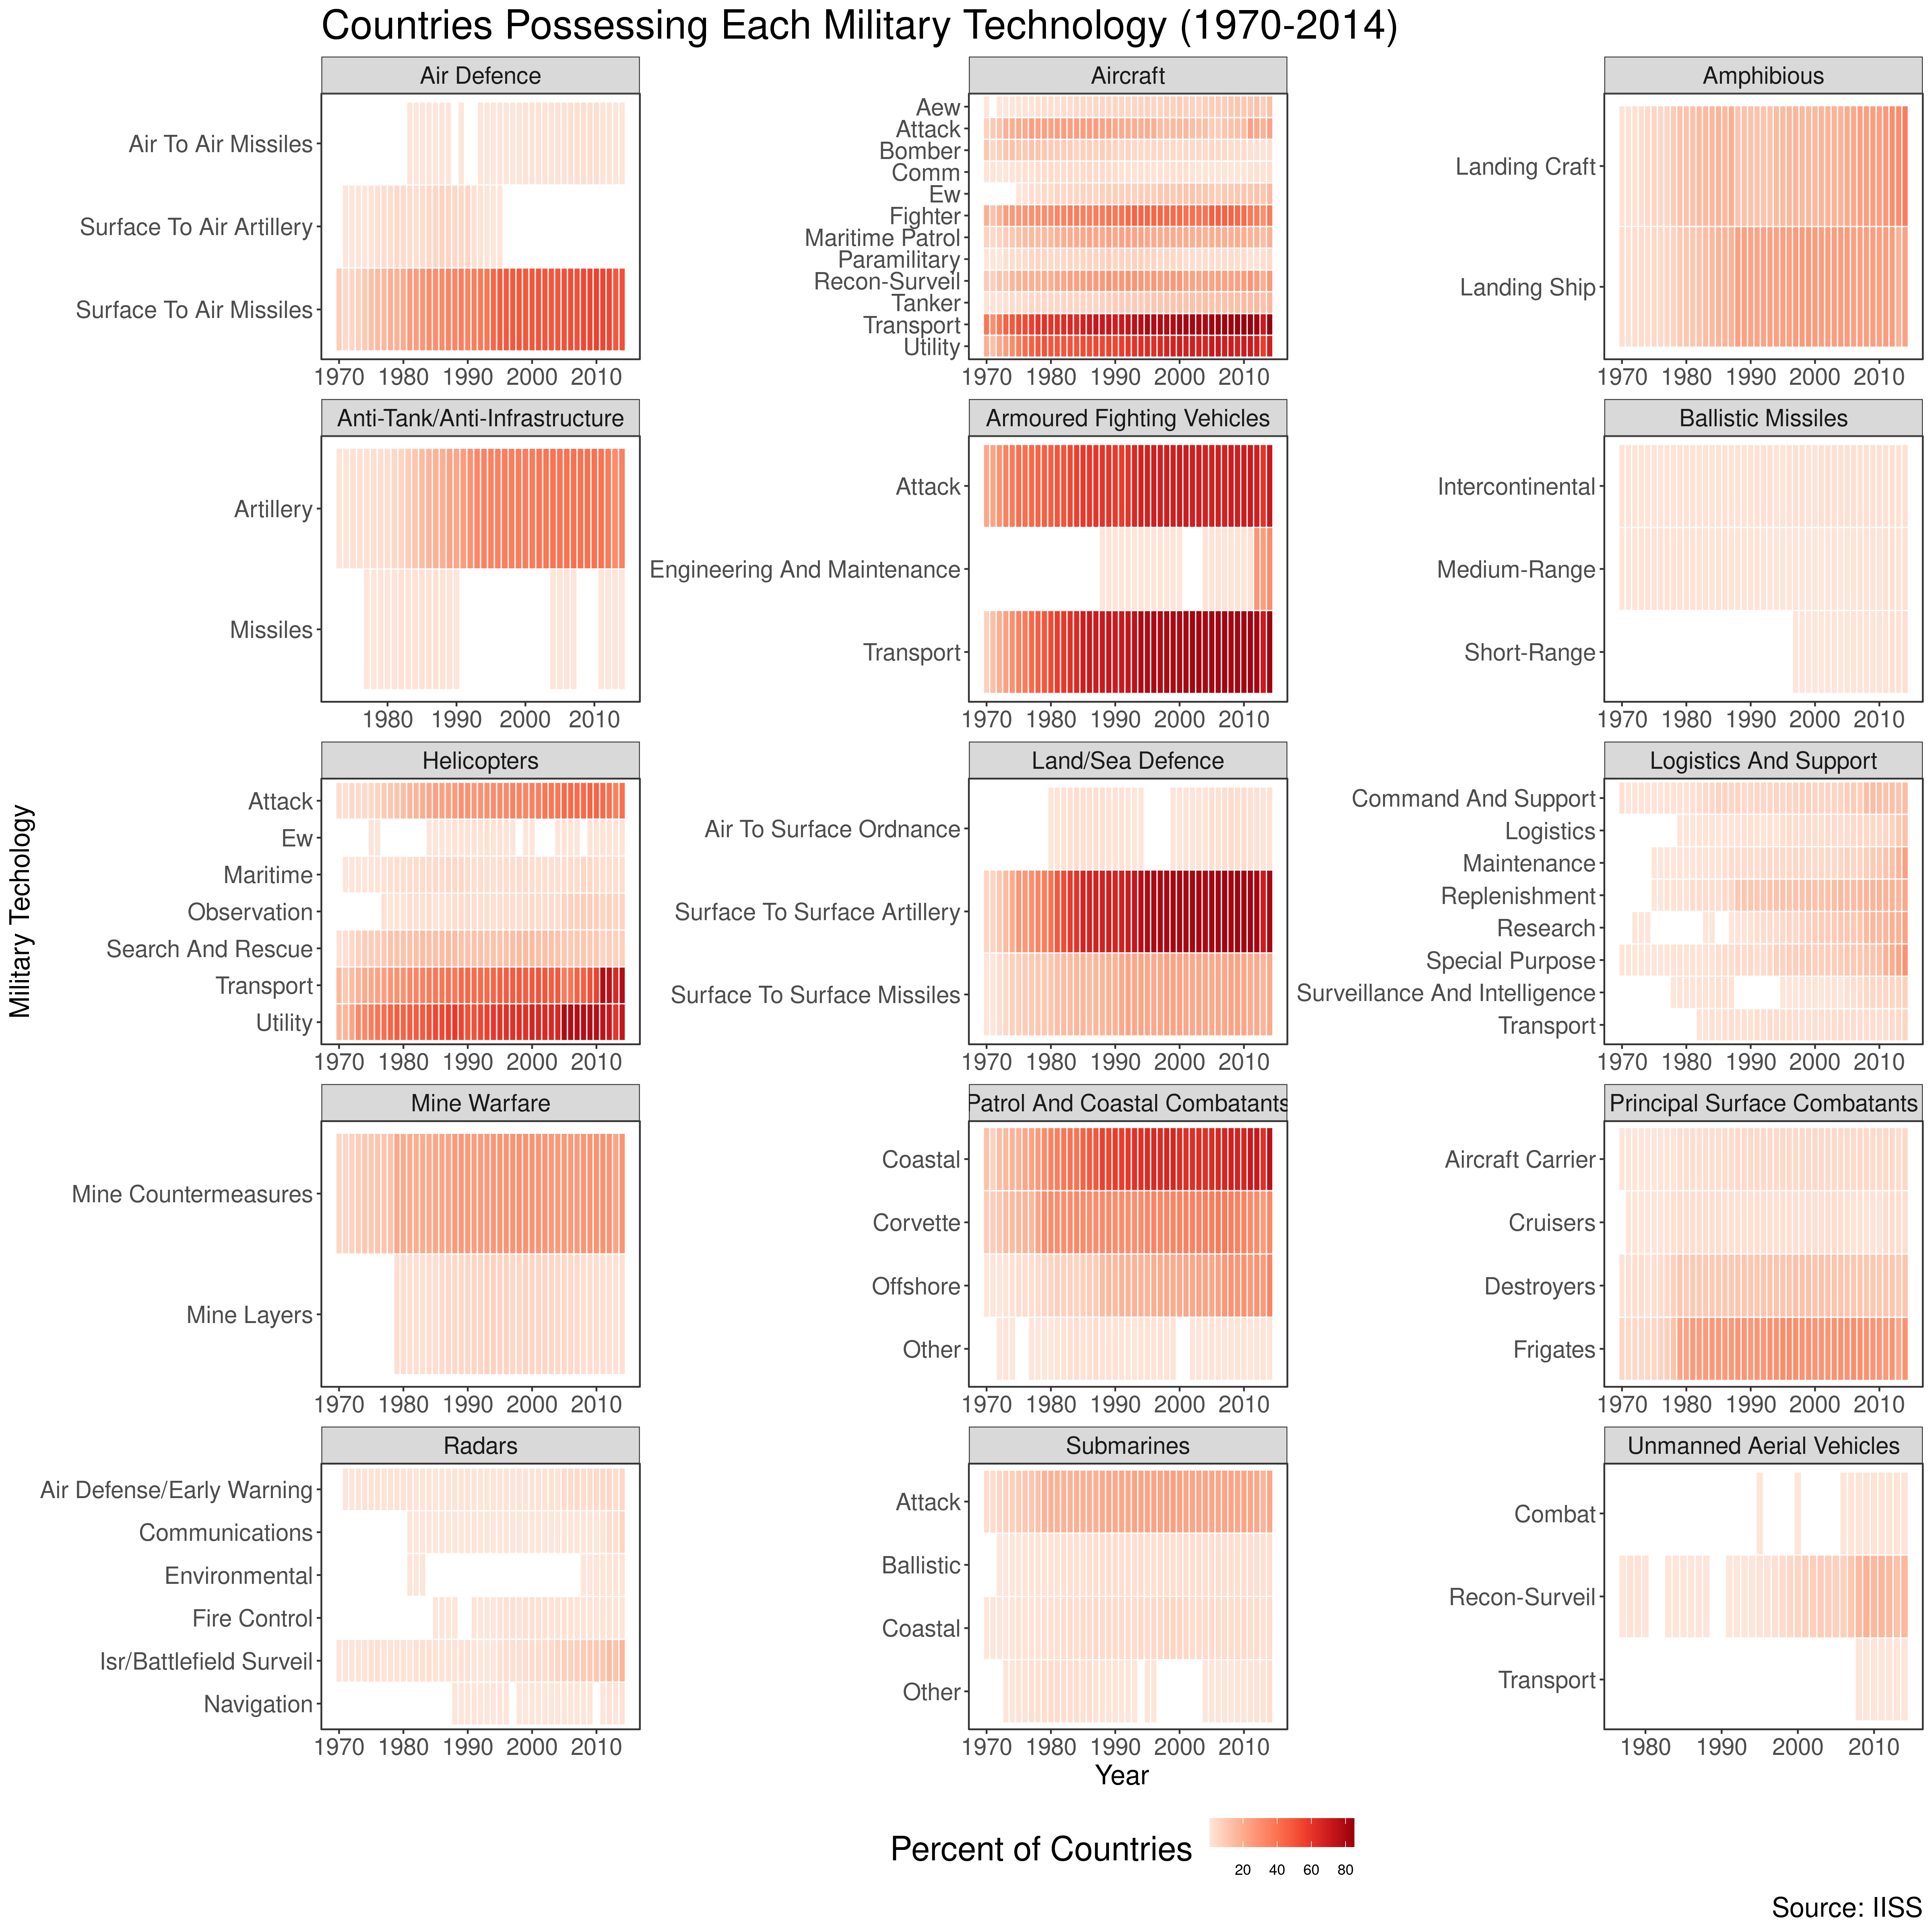
\includegraphics[width=1\linewidth]{figures/common_teks_per_year} \caption{The number of countries possessing at least one unit of each major military category of technology. Darker cells mean more countries possessed that technology in that year.}\label{fig:common-teks}
\end{figure}

Understanding these changes over time can also speak to questions of military effectiveness. For example, much has been written about the consequences of aerial bombing (Pape 1996; Allen and Martinez Machain 2017). Although this research has looked at cases where states used aerial bombing, it does not identify what states have the capacity to conduct aerial bombing or how that changes over time.\footnote{New data on combat aircraft has recently been produced by Saunders and Souva (2020).} Figure \ref{fig:aircraft} shows annual changes in the total number of military aircraft as well as changes in the annual average across all states. The end of the Cold War in 1991 is an important turning point in both respects. The number of total military aircraft in the world dropped from roughly 40,000 to just over 20,000 and the average military aircraft per country went from around 400 to just under 200. Why such a significant reduction in combat aircraft worldwide? Part of the explanation may be the Adapted Treaty on Conventional Armed Forces in Europe (CFE) which required NATO and the Warsaw Pact -- referred to in the CFE as the ``Groups of States'' -- to each maintain no more than 6,800 combat aircraft (Bolving 2000). This resulted in the destruction of 69,000 military units designated as Treaty Limited Equipment, with the Warsaw Pact destroying over 30\% of its arsenal and NATO destroying 5\% (McCausland 2012).

\begin{figure}
\centering
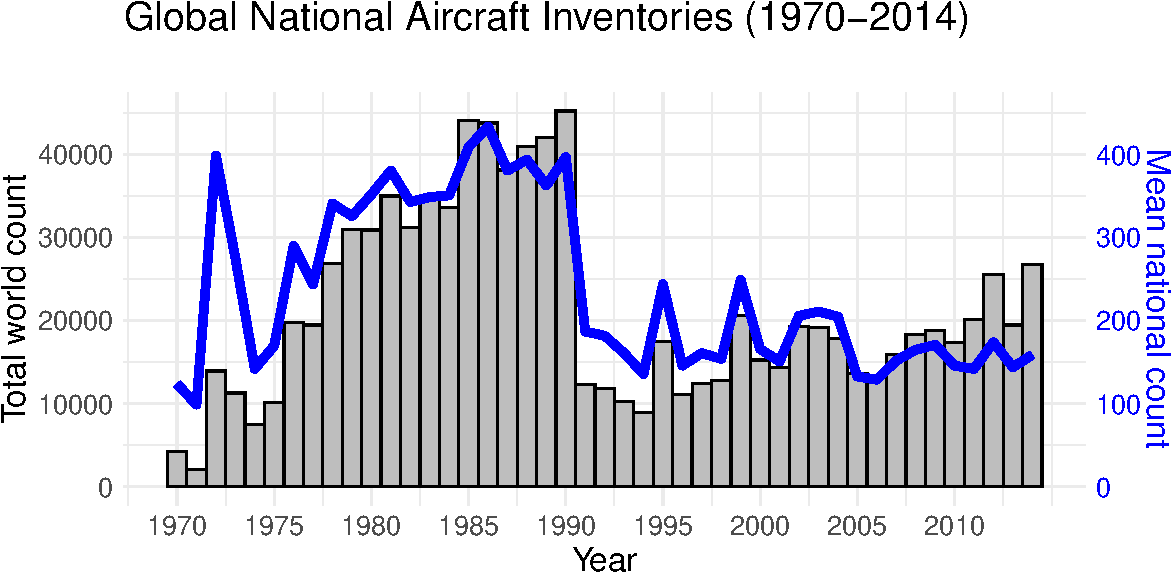
\includegraphics{figures/aircraft-1.pdf}
\caption{\label{fig:aircraft}Bars bars (left y-axis) represent the total number of military aircraft in the world in each year. The blue line (right y-axis) represents the average number of aircraft owned by each national military in each year.}
\end{figure}

\hypertarget{technological-trends-across-states}{%
\subsection{Technological Trends Across States}\label{technological-trends-across-states}}

Military capabilities differ in their purpose (Lindsay and Gartzke 2022). Some capabilities are most salient for states projecting power while others are relevant for territorial defense. All else being equal, what capabilities do states emphasize? Figure \ref{fig:lollipop-us} shows the distribution of US military capabilities relative to the world average at decade intervals. Not surprisingly, US capabilities generally dwarf those of the rest of the international system. But this is not universal, nor is the degree of US dominance constant. For much of the past half century, the United States has had fewer anti-tank/anti-infrastructure capabilities as well as fewer mine warfare capabilities than the average state. The 2022 Russian invasion of Ukraine has made this fact especially salient, as transfers of one third of the US anti-tank/anti-infrastructure weapons stockpile to Ukraine has prompted concern about the sustainability of such support (Cancian 2022).

Variation in the US distribution of capabilities could be explained by myriad factors. Perhaps geography makes mine warfare less valuable since the US primarily fights its wars far from home. Military capabilities have substitutes and complements, and it's possible that anti-tank/anti-infrastructure needs are adequately addressed with bombing aircraft and land defense missiles. Quantity is also not synonymous with quality, so it could be that the US is still more than sufficiently capable in these domains, but with fewer platforms. Whatever the theorized explanation, these new data now allows scholars to empirically examine claims about why states possess the distribution of military capabilities that they do.

\begin{figure}
\centering
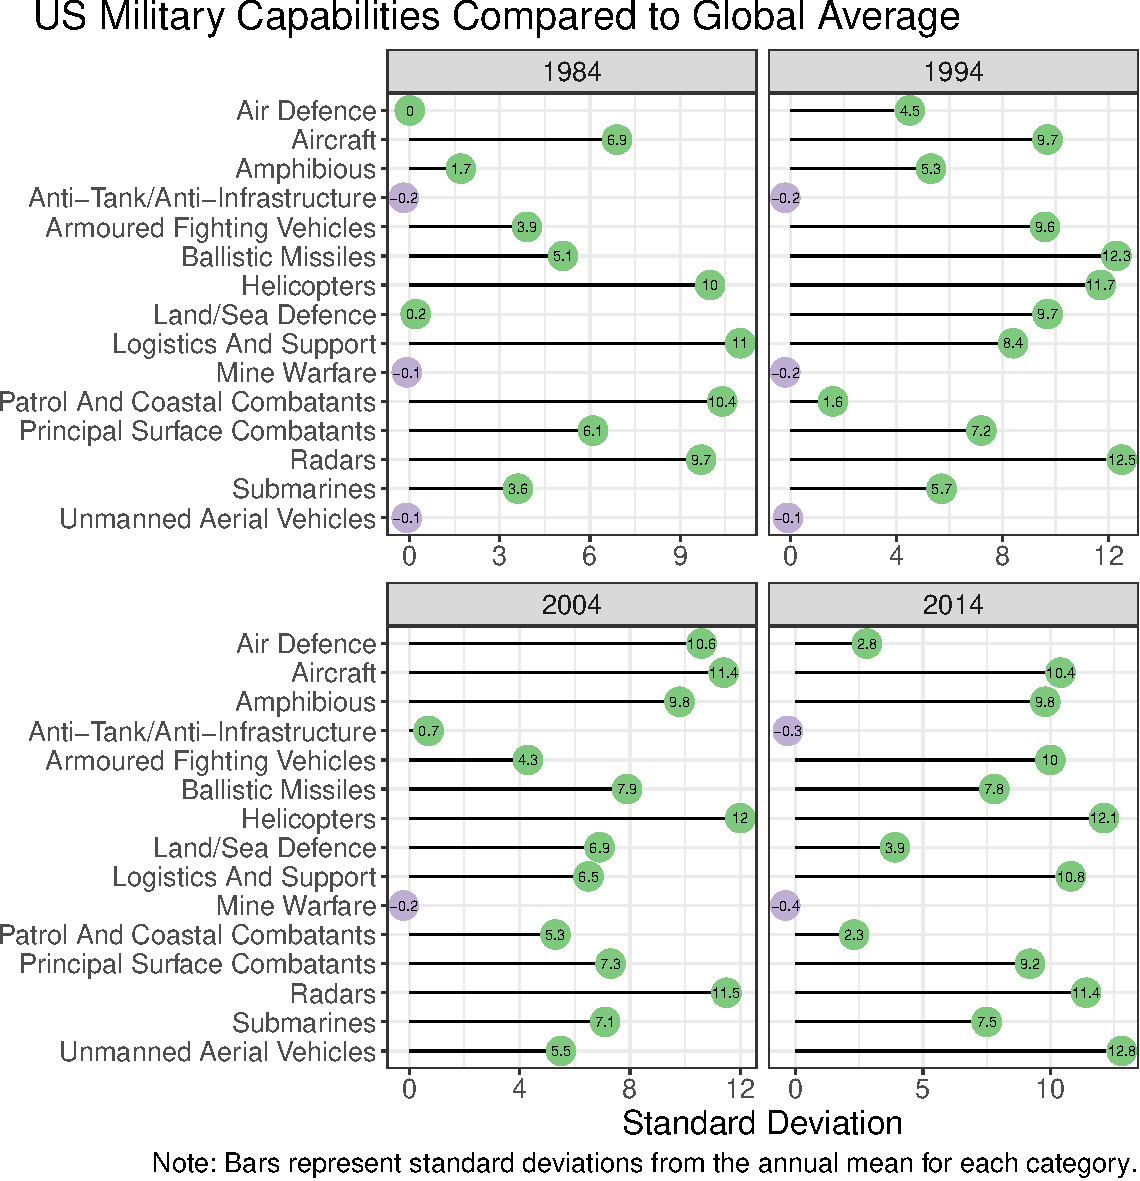
\includegraphics{figures/lollipop-us-1.pdf}
\caption{\label{fig:lollipop-us}Count of US military capabilities relative to other states in decade intervals. Each bar represents the standard deviation of the count of US capabilities relative to the world average. Colors represent positive and negative standard deviations.}
\end{figure}

When do states' military portfolios most closely mirror those of others? Some scholars argued socialization and competition under anarchy results in convergence, whereby states emulate the capabilities of the most powerful states in the international system (Waltz 1979 p 127; Resende-Santos 1996 p 196) while others have noted functional differentiation across allies who produce distinct, complementary military assets (Gannon 2021). Although there are instances of Cold War military planners falling prey to the homeopathy heuristic by embracing ``missile matching'' vis-à-vis their rivals (Kanwisher 1989), systematic evidence of similarity or difference across states' militaries has remained empirically untested. This claim is significant for scholars of international politics. If states mirror the military capabilities of others, then ``new and proven military methods, even if they are truly revolutionary, will have no lasting affect on the balance of international influence'' (Goldman and Andres 1999, p 83). This also has implications for what we know about security cooperation, with scholars cautioning that states imitating the military practices of their peers ``rarely resort to alliances for their security'' (Parent and Rosato 2015 p 52).

\emph{rDMC} allows the similarity of militaries around the world to be identified and quantitatively measured. Figure \ref{fig:country-clusters} shows the results of a k-means clustering analysis for all states in 2004 using binary values indicating whether a state possessed each of the 74 military technologies.\footnote{I exclude states with a population below 750,000 as done by Eyre and Suchman (1996) and Sechser and Saunders (2010). Other states are missing data because they were not yet sovereign states (South Sudan) or because data on military capabilities was not collected for states just after or still in a serious civil conflict (Congo).} A form of community detection, k-means clustering is an un-supervised learning algorithm that partitions the data into clusters of most-similar states using a gap statistic identifying the optimal number of groups (Tibshirani, Walther, and Hastie 2001).\footnote{This clustering method has been used for community detection of economic industries (Delgado, Porter, and Stern 2016), democratization patterns (Gleditsch and Ward 2006), and arms sales (Akerman and Seim 2014).} There are eight distinct clusters of countries that share significant commonality in the military capabilities they possess. States with militaries most similar to the US include great power rivals like Russia and China, some allies like France, Germany, and Spain, but not other allies like Poland, Sweden, and Canada. There is similarity across states in some geographic regions like Central Asia, but significant dissimilarity across states in other regions like Latin America.

\begin{figure}
\centering
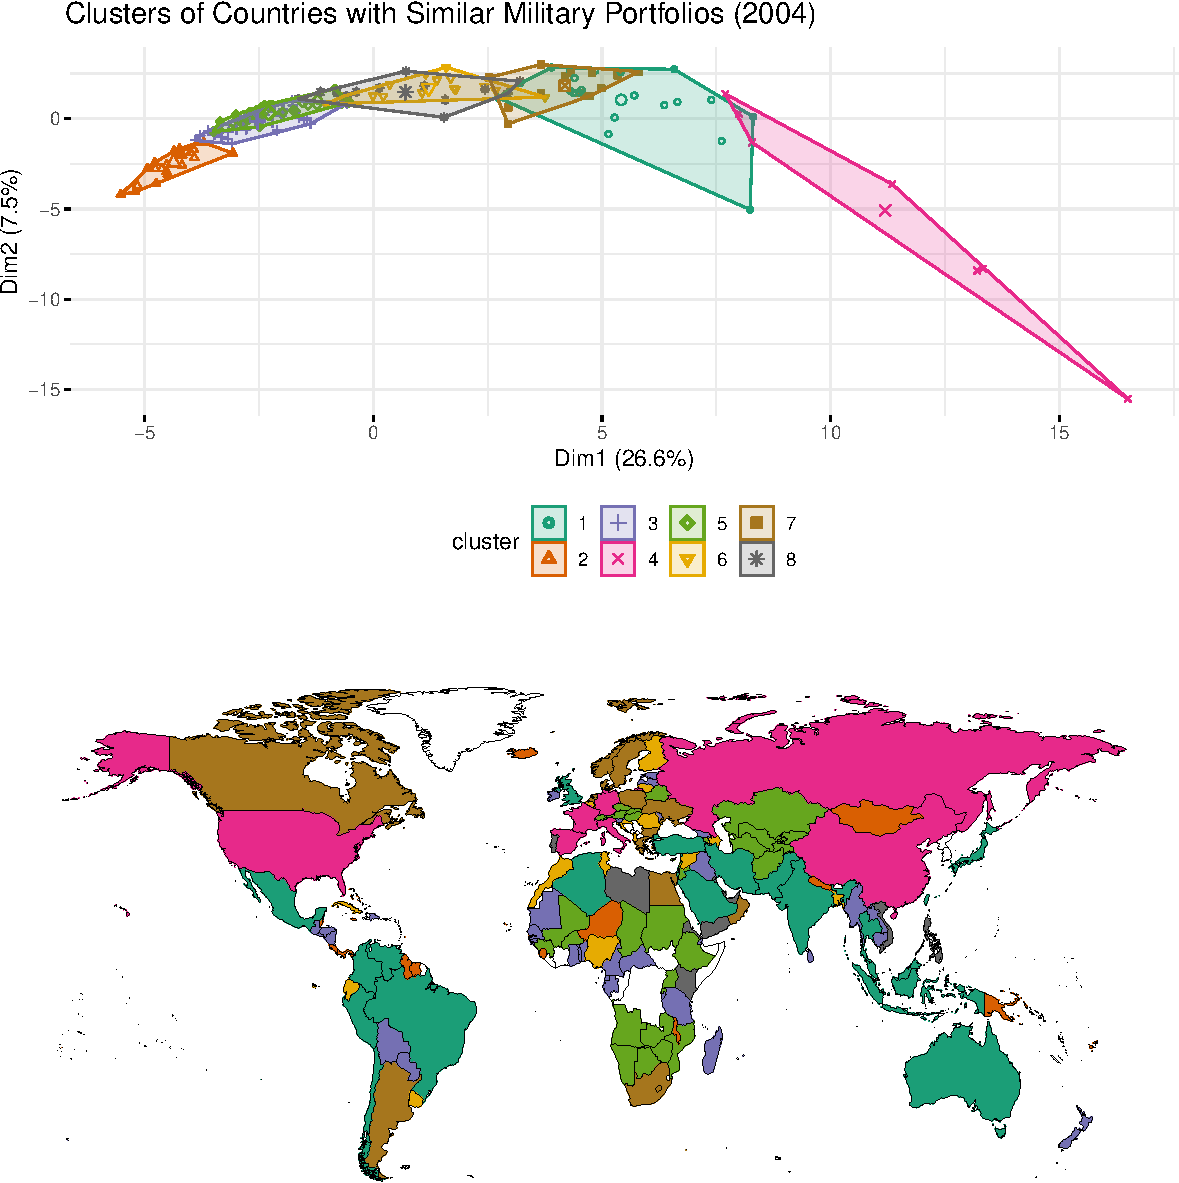
\includegraphics{figures/country-clusters-1.pdf}
\caption{\label{fig:country-clusters}K-means clustering showing the similarity of military technologies portfolios.}
\end{figure}

Cautioning that Figure \ref{fig:country-clusters} is a simplified example (a single year and using binary rather than count values), the results nonetheless demonstrate the utility of disaggregating military capabilities for identifying similarity in national defense portfolios and generating testable hypotheses concerning the relationship between military composition and factors like technological capacity, geography, threat environment, and conflict history. The fact there are differences in how even similarly-sized states arm themselves is prima facie evidence of the non-fungibility of material military power.

\hypertarget{conclusion}{%
\section{Conclusion}\label{conclusion}}

This paper merely represents version 1.0 of a dataset that has demonstrated value in helping us understand how states fight; efforts are already underway to expand the data temporally -- both beyond 2014 and further back than 1970, as well as increase the ease of using \emph{raw rDMC} by standardizing unit names across space and time. Even still, while much ink has been spilled debating the degree to which military technology matters, rDMC 1.0 can help the discussion productively shift to \emph{what} military technologies matter and \emph{how}. Understanding differences in the composition of military capabilities is vital to understanding military power precisely because these components are not homogeneous. Identifying the dimensions of this heterogeneity is a necessary precondition for explaining why states develop the weapons portfolio that they do as well as the consequences of armament decisions. The composition of military assets, rather than the defense dollars spent, are what truly matter for how well states deal with threats to their security because military spending itself does not create military power. Rather, that money must be translated into capabilities that allow for the exercise of power through a variety of distinct means.

To date, explanations of the causes or effects of variation in the composition of a state's military assets has been empirically limited because that data has not existed in a form conducive to systematic analysis. As a new, disaggregated dataset on the military capabilities states possessed over the past half century, \emph{rDMC} can help the broader scholarly community better explain how states arm, why, and to what effect.

\newpage

\hypertarget{references}{%
\section*{References}\label{references}}
\addcontentsline{toc}{section}{References}

\hypertarget{refs}{}
\begin{CSLReferences}{1}{0}
\leavevmode\vadjust pre{\hypertarget{ref-akerman_globalarmstrade_2014}{}}%
Akerman, Anders, and Anna Larsson Seim. 2014. {``The Global Arms Trade Network 1950\textendash 2007.''} \emph{Journal of Comparative Economics} 42 (3): 535--51. \url{https://doi.org/10.1016/j.jce.2014.03.001}.

\leavevmode\vadjust pre{\hypertarget{ref-albrecht_howkeepofficers_2018}{}}%
Albrecht, Holger, and Ferdinand Eibl. 2018. {``How to {Keep Officers} in the {Barracks}: {Causes}, {Agents}, and {Types} of {Military Coups}.''} \emph{International Studies Quarterly} 62 (2): 315--28. \url{https://doi.org/10.1093/isq/sqx085}.

\leavevmode\vadjust pre{\hypertarget{ref-alexander_countrysurveyxvii_2002}{}}%
Alexander, J., Alan B. King, and W. Robert. 2002. {``Country Survey {XVII}: {New} Zealand's Defence Policy.''} \emph{Defence and Peace Economics} 13 (4): 287--309. \url{https://doi.org/10.1080/10242690212355}.

\leavevmode\vadjust pre{\hypertarget{ref-allen_understandingimpactair_2017}{}}%
Allen, Susan Hannah, and Carla Martinez Machain. 2017. {``Understanding the Impact of Air Power.''} \emph{Conflict Management and Peace Science} 36 (5): 545--58. \url{https://doi.org/10.1177/0738894216682485}.

\leavevmode\vadjust pre{\hypertarget{ref-amara_unfulfilledpromisesimpact_2010}{}}%
Amara, Jomana, and Martins Paskevics. 2010. {``Unfulfilled {Promises}: {The Impact} of {Accession} on {Military Expenditure Trends} for {New NATO Members}.''} \emph{Comparative Strategy} 29 (5): 432--49. \url{https://doi.org/10.1080/01495933.2010.520988}.

\leavevmode\vadjust pre{\hypertarget{ref-bas_armsdiffusionwar_2012}{}}%
Bas, Muhammet A., and Andrew J. Coe. 2012. {``Arms {Diffusion} and {War}.''} \emph{Journal of Conflict Resolution} 56 (4): 651--74. \url{https://doi.org/10.1177/0022002712445740}.

\leavevmode\vadjust pre{\hypertarget{ref-beckley_emergingmilitarybalance_2017}{}}%
Beckley, Michael. 2017. {``The {Emerging Military Balance} in {East Asia}: {How China}'s {Neighbors Can Check Chinese Naval Expansion}.''} \emph{International Security} 42 (2): 78--119. \url{https://doi.org/10.1162/ISEC_a_00294}.

\leavevmode\vadjust pre{\hypertarget{ref-beckley_powernationsmeasuring_2018}{}}%
---------. 2018. {``The {Power} of {Nations}: {Measuring What Matters}.''} \emph{International Security} 43 (2): 7--44. \url{https://doi.org/10.1162/isec_a_00328}.

\leavevmode\vadjust pre{\hypertarget{ref-biddle_militarypowerexplaining_2005}{}}%
Biddle, Stephen. 2005. \emph{Military {Power}: {Explaining Victory} and {Defeat} in {Modern Battle}}. {Manas Publications}.

\leavevmode\vadjust pre{\hypertarget{ref-biden_bidenremarksmccain_2008}{}}%
Biden, Joseph. 2008. {``Biden's {Remarks} on {McCain}'s {Policies}.''} \emph{The New York Times}, September.

\leavevmode\vadjust pre{\hypertarget{ref-bolving_adaptedtreatyconventional_2000}{}}%
Bolving, Klaus. 2000. {``The {Adapted Treaty} on {Conventional Armed Forces} in {Europe} - {CFE} - {Considerations} Concerning {Baltic CFE-Membership}.''} \emph{Baltic Defence Review} 4 (2000): 31--66.

\leavevmode\vadjust pre{\hypertarget{ref-boniface_anneestrategique1995_1995}{}}%
Boniface, Pascal. 1995. \emph{L'année {Stratégique} 1995. {Les} Équilibres Militaire}. {Paris}: {Dunod for the Institut des Relations Internationales et Strategiques}.

\leavevmode\vadjust pre{\hypertarget{ref-brooks_creatingmilitarypower_2007}{}}%
Brooks, Risa, and Elizabeth Stanley, eds. 2007. \emph{Creating {Military Power}: {The Sources} of {Military Effectiveness}}. {Stanford University Press}.

\leavevmode\vadjust pre{\hypertarget{ref-brooks_risefallgreat_2016}{}}%
Brooks, Stephen G., and William C. Wohlforth. 2016. {``The {Rise} and {Fall} of the {Great Powers} in the {Twenty-first Century}: {China}'s {Rise} and the {Fate} of {America}'s {Global Position}.''} \emph{International Security} 40 (3): 7--53. \url{https://doi.org/10.1162/ISEC_a_00225}.

\leavevmode\vadjust pre{\hypertarget{ref-brzoska_reportingmilitaryexpenditures_1981}{}}%
Brzoska, Michael. 1981. {``The Reporting of Military Expenditures.''} \emph{Journal of Peace Research} 18 (3): 261--75.

\leavevmode\vadjust pre{\hypertarget{ref-cancian_willunitedstates_2022}{}}%
Cancian, Mark F. 2022. {``Will the {United States Run Out} of {Javelins Before Russia Runs Out} of {Tanks}?''} Commentary. {Center for Strategic \& International Studies}.

\leavevmode\vadjust pre{\hypertarget{ref-cappellazielinski_howstatespay_2016}{}}%
Cappella Zielinski, Rosella. 2016. \emph{How {States Pay} for {Wars}}. {Cornell University Press}.

\leavevmode\vadjust pre{\hypertarget{ref-carroll_predictionproxiespower_2019}{}}%
Carroll, Robert J., and Brenton Kenkel. 2019. {``Prediction, {Proxies}, and {Power}.''} \emph{American Journal of Political Science} 63 (3): 577--93. \url{https://doi.org/10.1111/ajps.12442}.

\leavevmode\vadjust pre{\hypertarget{ref-caverley_unitedstateshegemony_2007}{}}%
Caverley, Jonathan D. 2007. {``United {States Hegemony} and the {New Economics} of {Defense}.''} \emph{Security Studies} 16 (4): 598--614. \url{https://doi.org/10.1080/09636410701740825}.

\leavevmode\vadjust pre{\hypertarget{ref-caverley_militarytechnologyduration_2017}{}}%
Caverley, Jonathan D., and Todd S. Sechser. 2017. {``Military {Technology} and the {Duration} of {Civil Conflict}.''} \emph{International Studies Quarterly} 61 (3): 704--20. \url{https://doi.org/10.1093/isq/sqx023}.

\leavevmode\vadjust pre{\hypertarget{ref-crisher_navalpowerendogeneity_2017}{}}%
Crisher, Brian. 2017. {``Naval Power, Endogeneity, and Long-Distance Disputes.''} \emph{Research and Politics} 4 (1): 1--6.

\leavevmode\vadjust pre{\hypertarget{ref-crisher_powerseanaval_2014}{}}%
Crisher, Brian, and Mark Souva. 2014. {``Power at {Sea}: {A Naval Power Dataset}, 1865-2011.''} \emph{International Interactions} 40 (4): 602--29. \url{https://doi.org/10.1080/03050629.2014.918039}.

\leavevmode\vadjust pre{\hypertarget{ref-delgado_definingclustersrelated_2016}{}}%
Delgado, Mercedes, Michael E. Porter, and Scott Stern. 2016. {``Defining Clusters of Related Industries.''} \emph{Journal of Economic Geography} 16 (1): 1--38. \url{https://doi.org/10.1093/jeg/lbv017}.

\leavevmode\vadjust pre{\hypertarget{ref-douglass_churningbutterguns_2019}{}}%
Douglass, Rex W., and J Andrés Gannon. 2019. {``Churning {Butter} into {Guns}: {Identifying Latent Military Capacity}.''} Working \{\{Paper\}\}.

\leavevmode\vadjust pre{\hypertarget{ref-eyre_statusnormsproliferation_1996}{}}%
Eyre, Dana P., and Mark C. Suchman. 1996. {``Status, {Norms} and the {Proliferation} of {Conventional Weapons}: {An Institutional Theory Approach}.''} In \emph{The {Culture} of {National Security}: {Norms} and {Identity} in {World Politics}}, edited by Peter J. Katzenstein, 79--113. {New York, NY}: {Columbia University Press}.

\leavevmode\vadjust pre{\hypertarget{ref-fontanel_comparisonmilitarybudgets_1996}{}}%
Fontanel, Jacques. 1996. {``The Comparison of Military Budgets of the Eastern and Central {European} Countries.''} \emph{Defence and Peace Economics} 7 (2): 135--47. \url{https://doi.org/10.1080/10430719608404847}.

\leavevmode\vadjust pre{\hypertarget{ref-fordham_domesticpoliticsinternational_2002}{}}%
Fordham, Benjamin O. 2002. {``Domestic {Politics}, {International Pressure}, and the {Allocation} of {American Cold War Military Spending}.''} \emph{The Journal of Politics} 64 (1): 63--88. \url{https://doi.org/10.1111/1468-2508.00118}.

\leavevmode\vadjust pre{\hypertarget{ref-fordham_verysharpsword_2004}{}}%
---------. 2004. {``A {Very Sharp Sword}: {The Influence} of {Military Capabilities} on {American Decisions} to {Use Force}.''} \emph{Journal of Conflict Resolution} 48 (5): 632--56. \url{https://doi.org/10.1177/0022002704267935}.

\leavevmode\vadjust pre{\hypertarget{ref-gaibulloev_personnelcontributionsnonun_2015}{}}%
Gaibulloev, Khusrav, Justin George, Todd Sandler, and Hirofumi Shimizu. 2015. {``Personnel Contributions to {UN} and Non-{UN} Peacekeeping Missions: {A} Public Goods Approach.''} \emph{Journal of Peace Research} 52 (6): 727--42. \url{https://doi.org/10.1177/0022343315579245}.

\leavevmode\vadjust pre{\hypertarget{ref-gannon_usetheirforce_2021}{}}%
Gannon, J Andrés. 2021. {``Use {Their Force}: {Interstate Security Alignments} and the {Distribution} of {Military Capabilities}.''} PhD thesis, UC San Diego.

\leavevmode\vadjust pre{\hypertarget{ref-gannon_oneifland_2022}{}}%
---------. 2022. {``One If by Land, and Two If by Sea: {Cross-domain} Contests and the Escalation of International Crises.''} \emph{International Studies Quarterly} 66 (4).

\leavevmode\vadjust pre{\hypertarget{ref-gartzke_influenceseapower_2020}{}}%
Gartzke, Erik A., and Jon R. Lindsay. 2020. {``The {Influence} of {Sea Power} on {Politics}: {Domain-} and {Platform-Specific Attributes} of {Material Capabilities}.''} \emph{Security Studies} 29 (4): 601--36. \url{https://doi.org/10.1080/09636412.2020.1811450}.

\leavevmode\vadjust pre{\hypertarget{ref-gilli_spreadmilitaryinnovations_2014}{}}%
Gilli, Andrea, and Mauro Gilli. 2014. {``The {Spread} of {Military Innovations}: {Adoption Capacity Theory}, {Tactical Incentives}, and the {Case} of {Suicide Terrorism}.''} \emph{Security Studies} 23 (3): 513--47. \url{https://doi.org/10.1080/09636412.2014.935233}.

\leavevmode\vadjust pre{\hypertarget{ref-gleditsch_diffusioninternationalcontext_2006}{}}%
Gleditsch, Kristian Skrede, and Michael D. Ward. 2006. {``Diffusion and the {International Context} of {Democratization}.''} \emph{International Organization} 60 (4): 911--33.

\leavevmode\vadjust pre{\hypertarget{ref-goldman_systemiceffectsmilitary_1999}{}}%
Goldman, Emily O., and Richard B. Andres. 1999. {``Systemic Effects of Military Innovation and Diffusion.''} \emph{Security Studies} 8 (4): 79--125. \url{https://doi.org/10.1080/09636419908429387}.

\leavevmode\vadjust pre{\hypertarget{ref-greenhill_perilsprofilingcivil_2007}{}}%
Greenhill, Kelly M., and Solomon Major. 2007. {``The {Perils} of {Profiling}: {Civil War Spoilers} and the {Collapse} of {Intrastate Peace Accords}.''} \emph{International Security} 31 (3): 7--40. \url{https://doi.org/10.1162/isec.2007.31.3.7}.

\leavevmode\vadjust pre{\hypertarget{ref-horowitz_diffusionmilitarypower_2010}{}}%
Horowitz, Michael C. 2010. \emph{The {Diffusion} of {Military Power}: {Causes} and {Consequences} for {International Politics}}. {Princeton University Press}.

\leavevmode\vadjust pre{\hypertarget{ref-internationalinstituteforstrategicstudies_militarybalance_}{}}%
International Institute for Strategic Studies. n.d. \emph{The {Military Balance}}. {Oxford}: {Oxford University Press}.

\leavevmode\vadjust pre{\hypertarget{ref-kadercan_strongarmiesslow_2014}{}}%
Kadercan, Burak. 2014. {``Strong {Armies}, {Slow Adaptation}: {Civil-Military Relations} and the {Diffusion} of {Military Power}.''} \emph{International Security} 38 (3): 117--52. \url{https://doi.org/10.1162/ISEC_a_00146}.

\leavevmode\vadjust pre{\hypertarget{ref-kahn_whogetssmart_2022}{}}%
Kahn, Lauren, and Michael C. Horowitz. 2022. {``Who {Gets Smart}: {Explaining How Precision Bombs Proliferate}.''} \emph{Journal of Conflict Resolution}, July. \url{https://doi.org/10.2139/ssrn.3792071}.

\leavevmode\vadjust pre{\hypertarget{ref-kanwisher_cognitiveheuristicsamerican_1989}{}}%
Kanwisher, Nancy. 1989. {``Cognitive {Heuristics} and {American Security Policy}.''} \emph{Journal of Conflict Resolution} 33 (4): 652--75. \url{https://doi.org/10.1177/0022002789033004004}.

\leavevmode\vadjust pre{\hypertarget{ref-kupchan_natopersiangulf_1988}{}}%
Kupchan, Charles. 1988. {``{NATO} and the {Persian Gulf}: {Examining Intra-Alliance Behavior}.''} \emph{International Organization} 42 (2): 317--46.

\leavevmode\vadjust pre{\hypertarget{ref-kurth_politicaleconomyweapons_1972}{}}%
Kurth, James R. 1972. {``The {Political Economy} of {Weapons Procurement}: {The Follow-on Imperative}.''} \emph{The American Economic Review} 62 (1/2): 304--11.

\leavevmode\vadjust pre{\hypertarget{ref-lebovic_usingmilitaryspending_1999}{}}%
Lebovic, James. 1999. {``Using {Military Spending Data}: {The Complexity} of {Simple Inference}.''} \emph{Journal of Peace Research} 36 (6): 681--97.

\leavevmode\vadjust pre{\hypertarget{ref-leeds_alliancetreatyobligations_2002}{}}%
Leeds, Brett Ashley, Jeffrey Ritter, Sara Mitchell, and Andrew Long. 2002. {``Alliance {Treaty Obligations} and {Provisions}, 1815-1944.''} \emph{International Interactions} 28 (3): 237--60. \url{https://doi.org/10.1080/03050620213653}.

\leavevmode\vadjust pre{\hypertarget{ref-lieber_warengineersprimacy_2005}{}}%
Lieber, Keir A. 2005. \emph{War and the {Engineers}: {The Primacy} of {Politics Over Technology}}. {Cornell University Press}.

\leavevmode\vadjust pre{\hypertarget{ref-lindsay_politicsmanyother_2022}{}}%
Lindsay, Jon R., and Erik A. Gartzke. 2022. {``Politics by Many Other Means: {The} Comparative Strategic Advantages of Operational Domains.''} \emph{Journal of Strategic Studies} 45 (5): 743--76. \url{https://doi.org/10.1080/01402390.2020.1768372}.

\leavevmode\vadjust pre{\hypertarget{ref-ludeke_internationaltankdevelopment_2018}{}}%
Ludeke, Alexander. 2018. \emph{International {Tank Development From} 1970}. {Pen and Sword}.

\leavevmode\vadjust pre{\hypertarget{ref-lyall_ragemachinesexplaining_2009}{}}%
Lyall, Jason, and Isaiah Wilson. 2009. {``Rage {Against} the {Machines}: {Explaining Outcomes} in {Counterinsurgency Wars}.''} \emph{International Organization} 63 (1): 67--106. \url{https://doi.org/10.1017/S0020818309090031}.

\leavevmode\vadjust pre{\hypertarget{ref-mawdsley_armamentsdecisionmakingare_2018}{}}%
Mawdsley, Jocelyn. 2018. {``Armaments Decision-Making: {Are European} States Really Different?''} \emph{Comparative Strategy} 37 (4): 260--71. \url{https://doi.org/10.1080/01495933.2018.1497319}.

\leavevmode\vadjust pre{\hypertarget{ref-mccausland_europeaneurasiansecurity_2012}{}}%
McCausland, Jeffrey D. 2012. {``European/{Eurasian Security} and the {Treaty} on {Conventional Armed Forces} in {Europe}.''} {Strategic Studies Institute, US Army War College}.

\leavevmode\vadjust pre{\hypertarget{ref-officeofthesecretaryofdefense_militarysecuritydevelopments_2018}{}}%
Office of the Secretary of Defense. 2018. {``Military and {Security Developments Involving} the {People}'s {Republic} of {China} 2018.''} Annual \{\{Report\}\} to \{\{Congress\}\} 8-0F67E5F. {Department of Defense}.

\leavevmode\vadjust pre{\hypertarget{ref-pape_bombingwinair_1996}{}}%
Pape, Robert A. 1996. \emph{Bombing to {Win}: {Air Power} and {Coercion} in {War}}. {Cornell University Press}.

\leavevmode\vadjust pre{\hypertarget{ref-parent_balancingneorealism_2015}{}}%
Parent, Joseph M., and Sebastian Rosato. 2015. {``Balancing in {Neorealism}.''} \emph{International Security} 40 (2): 51--86. \url{https://doi.org/10.1162/ISEC_a_00216}.

\leavevmode\vadjust pre{\hypertarget{ref-perlo-freeman_monitoringmilitaryexpenditure_2017}{}}%
Perlo-Freeman, Sam. 2017. {``Monitoring Military Expenditure.''} {SIPRI}.

\leavevmode\vadjust pre{\hypertarget{ref-post_flyingfailcostly_2019}{}}%
Post, Abigail. 2019. {``Flying to {Fail}: {Costly Signals} and {Air Power} in {Crisis Bargaining}.''} \emph{Journal of Conflict Resolution} 63 (4): 869--95. \url{https://doi.org/10.1177/0022002718777043}.

\leavevmode\vadjust pre{\hypertarget{ref-resende-santos_anarchyemulationmilitary_1996}{}}%
Resende-Santos, Joâo. 1996. {``Anarchy and the Emulation of Military Systems: {Military} Organization and Technology in {South America}, 1870\textendash 1930.''} \emph{Security Studies} 5 (3): 193--260. \url{https://doi.org/10.1080/09636419608429280}.

\leavevmode\vadjust pre{\hypertarget{ref-saunders_commandskiesairpower_2020}{}}%
Saunders, Richard, and Mark Souva. 2020. {``Command of the {Skies}: {An Airpower Dataset}.''} \emph{Conflict Management and Peace Science} 37 (6): 735--55. \url{https://doi.org/10.1177/0738894219863348}.

\leavevmode\vadjust pre{\hypertarget{ref-schwartz_competeretreatglobal_2021}{}}%
Schwartz, Joshua A., and Michael C Horowitz. 2021. {``To {Compete} or {Retreat}? {The Global Diffusion} of {Precision Strike}.''} Working \{\{Paper\}\}.

\leavevmode\vadjust pre{\hypertarget{ref-sechser_armyyouhave_2010}{}}%
Sechser, Todd S., and Elizabeth N. Saunders. 2010. {``The {Army You Have}: {The Determinants} of {Military Mechanization}, 1979\textendash 2001.''} \emph{International Studies Quarterly} 54 (2): 481--511. \url{https://doi.org/10.1111/j.1468-2478.2010.00596.x}.

\leavevmode\vadjust pre{\hypertarget{ref-souva_materialmilitarypower_2023}{}}%
Souva, Mark. 2023. {``Material {Military Power}: {A Country-Year Measure} of {Military Power}, 1865-2019.''} \emph{Journal of Peace Research}.

\leavevmode\vadjust pre{\hypertarget{ref-stanton_terrorismcontextcivil_2013}{}}%
Stanton, Jessica A. 2013. {``Terrorism in the {Context} of {Civil War}.''} \emph{The Journal of Politics} 75 (4): 1009--22. \url{https://doi.org/10.1017/S0022381613000984}.

\leavevmode\vadjust pre{\hypertarget{ref-tibshirani_estimatingnumberclusters_2001}{}}%
Tibshirani, Robert, Guenther Walther, and Trevor Hastie. 2001. {``Estimating the Number of Clusters in a Data Set via the Gap Statistic.''} \emph{Journal of the Royal Statistical Society: Series B (Statistical Methodology)} 63 (2): 411--23. \url{https://doi.org/10.1111/1467-9868.00293}.

\leavevmode\vadjust pre{\hypertarget{ref-vancreveld_lessmeetseye_2005}{}}%
van Creveld, Martin. 2005. {``Less Than {Meets} the {Eye}.''} \emph{Journal of Strategic Studies} 28 (3): 449--52. \url{https://doi.org/10.1080/01402390500137341}.

\leavevmode\vadjust pre{\hypertarget{ref-waltz_theoryinternationalpolitics_1979}{}}%
Waltz, Kenneth. 1979. \emph{Theory of {International Politics}}. {Waveland Press}.

\leavevmode\vadjust pre{\hypertarget{ref-whitten_butterygunswelfare_2011}{}}%
Whitten, Guy D., and Laron K. Williams. 2011. {``Buttery {Guns} and {Welfare Hawks}: {The Politics} of {Defense Spending} in {Advanced Industrial Democracies}.''} \emph{American Journal of Political Science} 55 (1): 117--34. \url{https://doi.org/10.1111/j.1540-5907.2010.00479.x}.

\leavevmode\vadjust pre{\hypertarget{ref-wohlforth_stabilityunipolarworld_1999}{}}%
Wohlforth, William C. 1999. {``The {Stability} of a {Unipolar World}.''} \emph{International Security} 24 (1): 5--41. \url{https://doi.org/10.1162/016228899560031}.

\leavevmode\vadjust pre{\hypertarget{ref-zarzecki_armsdiffusionspread_2002}{}}%
Zarzecki, Thomas W. 2002. \emph{Arms {Diffusion}: {The Spread} of {Military Innovations} in the {International System}}. {Psychology Press}.

\end{CSLReferences}

\end{document}
